% Document class options:
% =======================
%
% serif: Sets the body font to be serif.
%
% twocolumn: Sets the body text in two - column layout.
%
% Fill in the type of article here.
% empirical
  % reflection
  % meta
  % rga
  % editorial
  %
% Using other bibliography styles:
% =======================
% authordate = APA
  % number =[1]
  %
    \documentclass[twocolumn,  rga,issue, numeric]{jote-new-article}


  %%% Add the bibliography, make sure it's in the same directory
\addbibresource{valentini.bib}
%%% Add additional packages here if required.Usually not needed, except when doing things with figures and tables, god help you then

  % This package is for generating Lorem Ipsum, usage: \lipsum[X] where X is the Xth paragraph of lorem ipsum.OR use[1 - 5] to generate the first five, etc.


%%% TODO: Make this a 1 - 5 option scale to reduce the chance of mistyping

  % Enter the title, in Title Case Please
    % Try to keep it under 3 lines
\jotetitle{Neurological Markers of Maladaptive Brain Activity in Fibromyalgia and their Relationship with Treatment Effectiveness}

% List abbreviations here, if any.Please note that it is preferred that abbreviations be defined at the first instance they appear in the text, rather than creating an abbreviations list.
%\abbrevs{
%  ABC, a black cat; DEF, doesn't ever fret; GHI, goes home immediately.}

    % Include full author names and degrees, when required by the journal.
% Use the \authfn to add symbols for additional footnotes and present addresses, if any.Usually start with 1 for notes about author contributions; then continuing with 2 etc if any author has a different present address.
% Format: \author[1, 2]{FirstName LastName} \author[2]{...}
  \author[1]{Elia Valentini}

    % Fill it in again for the PDF metadata.Lame workaround but it works
      % Format: \authorone{...} \authortwo{...}
  \authorone{Elia Valentini}

    % List the contribution effort here, they will be listed at the end of the page
      % List the acknowledgments.If there is no companion piece, this is listed below the author info
        %\acknowledgments{Author Two would like to thank Author One for doing all the work while they could slack off.}
% List possible conflict of interest.Will default to saying no conflict exists.
%\interests{Author One was paid for by Big Failed Experiment}
% List funding
    %\funding{}
% Include full affiliation details for all authors
\affil[1]{Department of Psychology and Centre for Brain Science, University of Essex}

    % List the correspondence email of the main correspondent
 % \corraddress{corraddressmarker}
  \corremail{\href{evalent@essex.ac.uk}{evalent@essex.ac.uk}}

% Optionally list the present address of one of the authors
    %\presentadd[\authfn{2}]{Department, Institution, City, State or Province, Postal Code, Country}

% Fill in the DOI of the paper

    % Always starts with '10.36850/' and is suffixed with one of the following plus a number
      % e  : empirical
        % r  : reflection
          % mr : meta - research
            % rga: rejected grant application
              % ed : editorial
              %
  \paperdoi{10.36850/rga5}

% Include the name of the author that should appear in the running header
  \runningauthor{Valentini}

% The name of the Journal
  \jname{Journal of Trial \& Error}

% The year that the article is published
  \jyear{2021}
\jissue{1}
\jvolume{2}
\setcounter{page}{92-98}
\setcounter{page}{92}
% The Volume Number
    %\jvolume{Fall}

% The website that's listed in the bottom right
  \jwebsite{
    https://www.jtrialerror.com}

%%% Only \paperpublished is necessary, any combination of the other two is possible

      % When the paper was received
        % Format: 1 January, 1900
    \paperreceived{10 November, 2021}
% When the paper was accepted
      % Format: 1 January, 1900
    \paperaccepted{22 November, 2021}
% When the paper will be published
      % Format: 1 January, 1900
    \paperpublished{31 December, 2021}
    \paperissued{3 March, 2022}
% When the paper is published but in YYYY - MM - DD format, for the crossmark button
    \paperpublisheddate{2021-12-31}

      % Reflection and Empirical articles have each other as companion pieces.Add the DOI, Title, and Abstract of the respective Companion piece here

        %%% Abstrac\u
        \usepackage{balance}

    \keywordsabstract{fibromyalgia, pain, EEG, cytokines,
neuroinflammation, brain}
\rgainfo{Academy of Medical Sciences -- Springboard Round 4 2018 - SBF004\textbackslash1012}

%%%%%%%%%%%%%%%%%%%%%%%%%%%%%%%%%%%%%%%%%%%%%%%%%%%
% Document Starts
      %%%%%%%%%%%%%%%%%%%%%%%%%%%%%%%%%%%%%%%%%%%%%%%%%%%

    \begin{document}
%%% This starts the frontmatter, which includes everything that's on the front page execpt the text of the article
    \begin{frontmatter}
    \maketitle
      % Type your abstract between these things.Max 250 words.Be sure to include the \noindent, looks bad otherwise
    \begin{abstract}
Chronic pain (CP) is estimated to affect at least one-third of the
population in the United Kingdom. Fibromyalgia (FM) is one of the most
disabling CP conditions. Epidemiological research suggests its global
prevalence to be between 2-8\%. The unknown pathogenesis, lack of
biological markers to monitor its development, and lack of successful
treatment make FM a crucial target of pre-clinical research.

The goal of this project is twofold. The project aims to 1) identify
robust neurological markers (i.e., electrochemical brain activity) by
applying a combination of advanced electroencephalography (EEG) signal
processing (i.e., functional connectivity of oscillatory activity) and
neuroinflammatory (NI) responses (i.e., estimation of pro-inflammatory
cytokines intake), through which 2) characterizing successfully and
unsuccessfully treated FM patients (compared to age-matched healthy
controls). These measures, seldom combined, have been successfully
applied to the study of psychiatric conditions and sleep. Crucially, the
identification of neurological markers at rest and during arousing
sensory stimulation will allow us to estimate the relationship between
these neurological markers and treatment effectiveness. This proposal is
important because it aims to generate a robust pre-clinical neurological
tool to identify FM and its relationship with measures of treatment
effectiveness. The successful identification of neurological markers
will improve the assessment of the development of maladaptive changes in
FM and will kick-start further research on treatment effectiveness.

This project is of great medical relevance as it will identify
pathological signatures of FM that can then inform research on etiology
and treatment of this condition.
    \end{abstract}
    \end{frontmatter}











\section{Research proposal}



\subsubsection{The institution of employment at time of application}


University of Essex


\subsubsection{Prospective host institution}


University of Essex


\subsubsection{Main field}


Neuroscience


\subsubsection{Other fields}


Pain


\subsection{Description of the proposed research}



\subsubsection{Overall aim and key objectives}


Pain is a major burden for our society. In the United Kingdom, chronic
pain is estimated to affect between one-third and one-half of the
population. This impressive figure is likely to increase with the
progressive ageing of the population \cite{Fayaz2016}. A recent survey
revealed that 19\% of the European population have experienced moderate
or severe pain for at least six months duration and at least twice a
week. About 40\% of these people report insufficient pain treatment,
both pharmacological and non-pharmacological \cite{Breivik2006}.

Fibromyalgia (FM) is a chronic pain syndrome affecting the central,
autonomic, endocrine, and immune systems, often leading to an intense
state of suffering and disability. Epidemiological research suggests its
global prevalence to be between 2-8\% with a predominant female/male
ratio \cite{Clauw2014}. FM diagnosis is currently accomplished through
clinical assessment, as no validated biological markers have been
identified. Its diagnosis relies on the assessment of subjective
dimensions such as pain, fatigue, and sleep quality using the Symptom
Severity (SS) and Widespread Pain Index (WPI) \cite{Wolfe2010}. As a
result, there is large variability between diagnoses \cite{Walitt2016}.
Research suggests that central nervous system sensitization is
considered the hallmark of the pathological trajectory of FM, leading to
an increased gain in pain and sensory processing \cite{Sluka2016}.

Neuroimaging studies using functional magnetic resonance imaging show
altered brain communication between cerebral regions in FM patients,
namely intrinsic resting state connectivity \cite{Napadow2012,Napadow2010}.
Further evidence points to inflammatory mechanisms triggered by the
activation of mast cells \cite{Chatterjea2015}. Current targets of
investigation in FM are IL-1, IL-6, and IL-8 and the tumor necrosis
factor (TNF) \cite{Theoharides2015}. Despite increased investigation into
the relationship between increase in cytokines synthesis and increased
excitability of the brain \cite{Galic2012}, no research project has
studied them in combination with EEG activity in FM.

Importantly, many FM patients report dissatisfaction with the available
treatments \cite{Lauche2013}. Management strategies for FM vary and
the effect size of most treatments is modest \cite{Macfarlane2016}.
Therefore, not only is there a lack of diagnostic tools to effectively
identify FM, but there is also high variability and limited
effectiveness of its treatment. By ``treatment effectiveness'', the
project refers to how beneficial a FM treatment is in everyday life
compared to no treatment, assessed by a series of outcome measures, such
as pain, fatigue, mood and anxiety, sleep quality, daily functioning,
and well-being \cite{Carville2008}. An effective treatment is one that
is likely to reduce/improve the aforementioned symptoms. It follows that
there may be substantial differences in brain and neuroinflammatory (NI)
correlates between healthy and FM individuals, as well as between FM
individuals who are experiencing an effective treatment compared to
those who have not had a successful therapy. Neither issue has received
enough investigation so far.


\subsubsection{Research plan}


\noindent\paragraph{\noindent Design}


The project addresses the following question: Can we exploit functional
connectivity of oscillatory EEG activity and pro-inflammatory cytokines
intake as pre-clinical neurological markers and treatment effectiveness
in FM? In other words, this project aims to extend existing knowledge on
abnormal brain processing and enhanced NI activity in FM. Another
element of this project's originality comes from our attempt to provide
a characterization of neurological patterns in FM individuals undergoing
effective vs. ineffective treatment (compared to age-matched healthy
controls). Thus, there will be two specific objectives: 1) to identify
distinct EEG and NI markers of FM; 2) to characterize the EEG and NI
profile associated with treatment effectiveness in FM. FM patients will
be assigned to two different outcome groups based on scores in pain,
fatigue, mood and anxiety, sleep quality, daily functioning, and
well-being. The project will then measure their neurological
trajectories prior to and 3 months after the start of their treatment
(see tasks in Fig. 1 timeline) using a combination of advanced EEG
signal processing and NI responses. These measures, seldom combined,
have been successfully applied to the study of psychiatric conditions
and sleep. In the meantime, EEG responses will also be recorded in a
group of healthy age-matched individuals. Therefore, the research design
will consist of three groups: FM patients with effective treatment
(Feff), FM patients with ineffective treatment (Fineff), and age-matched
healthy controls (Ctrl). Treatment effectiveness will be assessed based
on reductions in current symptoms compared to the pre-treatment. By
doing so, the project essentially asks whether discriminatory patterns
of EEG and NI can be detected not only between Ctrl and FM patients, but
also between Feff and Fineff.

It is estimated that at least 20 participants per each experimental
group will enter the study (in line with a power estimate based on
previous neuroimaging studies). Participants will be all female (because
of the large predominance of the disease in the female population) and
selected on the basis of stringent exclusion
criteria \cite{Napadow2010}. The control group of healthy age-matched
individuals (n=30) will outnumber the experimental groups to increase
the accuracy of the findings.

\begin{figure*}
\captionsetup{width=\dimexpr \linewidth+\fullwidthlen\relax}
\begin{fullwidth}
 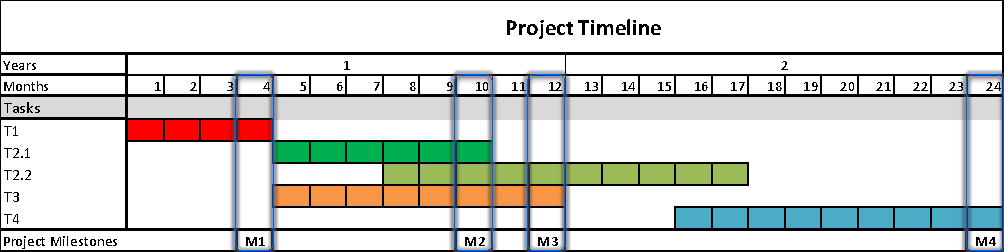
\includegraphics[width=\linewidth]{media/fig1.pdf}
  \end{fullwidth}
 \begin{adjustwidth}{-.5\fullwidthlen}{}
  

\caption{\textbf{Project timeline}.  The scientific objectives of the project will be achieved through 4 Tasks (T) and verified at 4 Milestones (M). The first month of the project will involve the PI and the PDRA in collecting relevant clinical data and self-report questionnaire scores of Fibromyalgia (FM) patients who just started a therapy (T1, red). These will be collected again after 3 months to determine which of the patients are benefitting from their therapy (i.e., showing reduction in symptoms). Based on this assessment, participants will be assigned to either the effective treatment (Feff) group, or to the ineffective treatment (Fineff) group (M1). Both groups will undergo a first experimental session (T2.1, green) whereby symptoms will be recorded, blood sampling for extraction of neuroinflammatory (NI) indexes will be performed, and electroencephalography (EEG) data will be obtained at month 10 (M2). Symptoms and EEG measurements will also be collected in age-matched healthy controls (Ctrl) which will start in parallel with T2.1 (T3, orange) but will proceed at lower priority and end at month 12. A minimum lapse of 3 months will be interleaved before a FM patient goes through a second session of symptoms, NI, and EEG data collection (T2.2, light green), wherein the same staff will be involved. T2.2 will initially be paced slowly because of the overlapping T2.1 and T3. The last task (T4, blue) will start at month 16 and will consist of statistical analysis of self-report, NI, and EEG data for the three groups, and preparation of the findings for dissemination in the shape of conference presentations and scientific articles (M4). T4 will involve the PDRA, the PI and the scientific collaborator (Dr. Metodiev).}
\end{adjustwidth}
\end{figure*}

\noindent\paragraph{\noindent Methodology}



\subparagraph{Self report measures}


The main criterion for participation will be a diagnosis of FM and the
final score in the SS and WPI. Participants who do not meet the
inclusion criterion of WPI \textgreater{} 7 and SS \textgreater{} 5 or
WPI between 3-6 and SS \textgreater{} 9 will be not allowed to enter the
study, as they would not clinically classify as FM patients. Patients
who enter the study will then be submitted to a series of measures. The
project will use the Fibromyalgia Impact Questionnaire (FIQ), which is a
multidimensional self-administered instrument that covers the following
dimensions: physical functioning (11 items), well-being (1 item), work
situation (2 items), pain (1 item), fatigue/sleep (2 items), stiffness
(2 items), and psychological symptoms (2 items). The Patient Health
Questionnaire (PHQ-9) will be used to investigate current disposition to
depressive symptoms \cite{Kroenke2002} and the General Anxiety Disorder
questionnaire \cite{Spitzer2006} will be used to assess disposition to
anxiety. In addition, participants will complete the Pain
Catastrophizing Scale (PCS) \cite{Sullivan1995}, a questionnaire that
measures the cognitive/emotional attitude towards pain, and the
Warwick-Edinburgh Mental Well-being Scale (WEMWBS) \cite{Tennant2007}
to quantify well-being.


\subparagraph{EEG recording and data analysis}

I have extensive experience in EEG techniques and pain
research \cite{Legrain2012,Torta2017}. The project will take advantage of my
collaboration with Fibromyalgia Research UK to recruit FM patients and
with the molecular biology lab led by Dr. Metodiev to extract cytokines
from participants' blood samples and quantify them for each participant.
As FM is known to be associated with abnormal processing in both rest
and stimulation states \cite{Sluka2016}, EEG activity will be measured
at rest and during repetition of vibrotactile stimuli at both T0 and T1.
This approach, while providing us with a measure of central
sensitization of the somatosensory system, will not cause pain.
Intrinsic oscillatory activity with eyes opened and eyes closed at rest
will be analyzed, as well as stimulus-related activity. Both traditional
power spectra analysis and functional connectivity approaches will be
used.

More precisely, I will test whether 1) patients who did not achieve an
effective treatment will show reduced EEG synchronization and increased
fronto-parietal connectivity compared to healthy controls and patients
who obtained an effective treatment; 2) patients who did achieve an
effective treatment will show increased EEG synchronization and
decreased mid-cingulate/premotor connectivity (see Fig. 2 for
preliminary data) on T1 compared to T0 (and vice versa for patients who
did not obtain effective treatment); 3) this effect will be predicted by
increased cytokine concentration for patients who did not achieve
effective treatment (and predicted by reduced cytokine intakes in
patients who obtained an effective treatment).

\begin{figure*}
  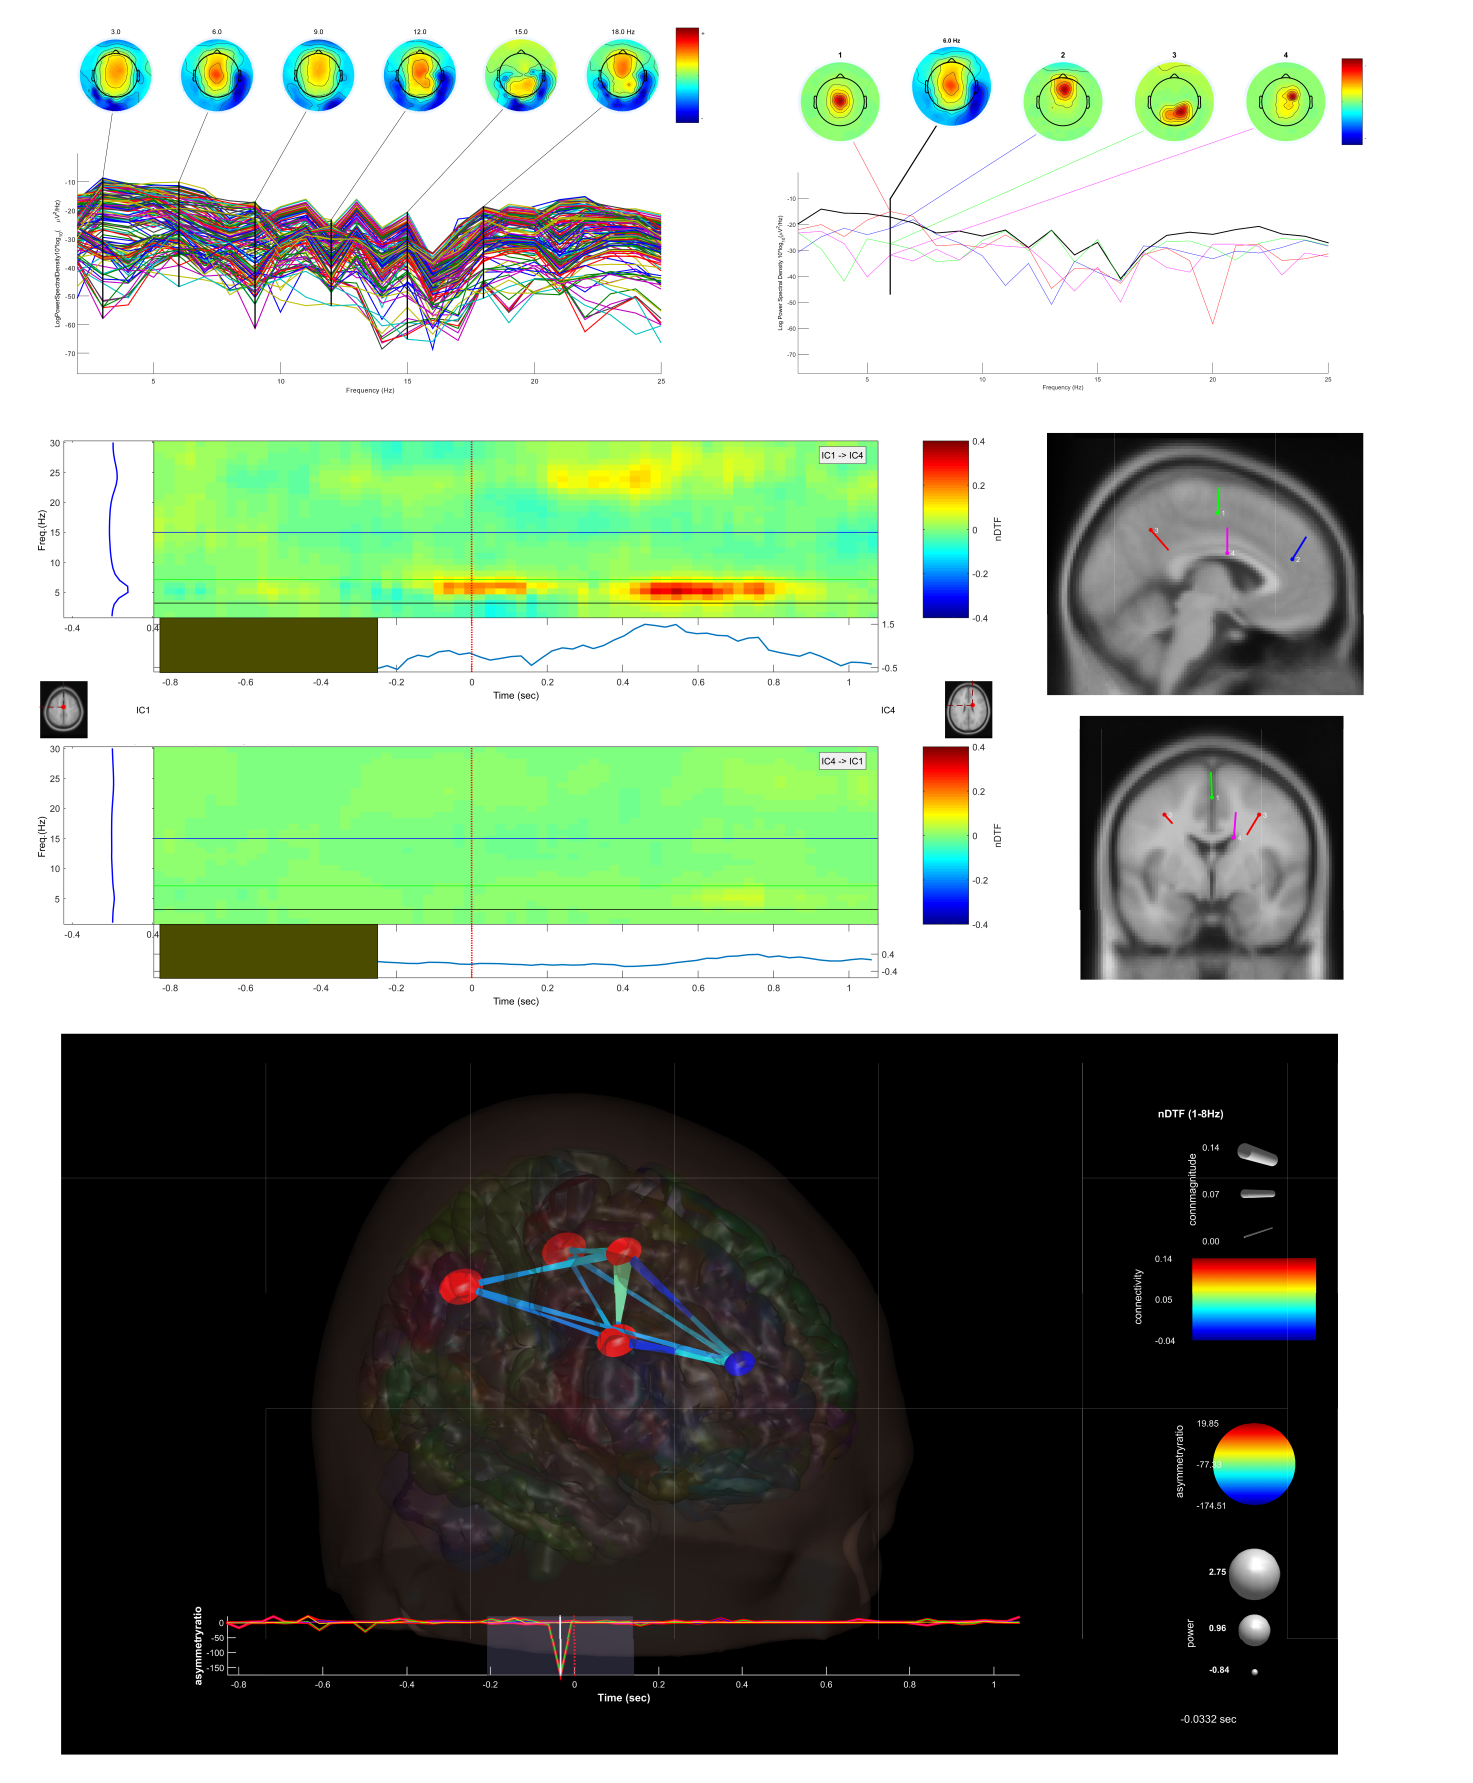
\includegraphics[width=.9\linewidth]{./media/fig2.png}
  
  \caption{\textbf{Functional connectivity analysis}. Example of a preliminary test of connectivity analysis on a sample of 20 healthy individuals administered with the somatosensory repeated stimulation mentioned in the current project. The left plot in the upper panel shows the frequency spectrum of EEG power (1-25 Hz) across single trials in the sample. The plot on the right provides independent components (as specified by the independent component analysis) of the EEG power at 6 Hz. This activity is well-known to represent the vertex EEG response commonly elicited by salient sensory stimuli.
     The left plot in the centre panel shows the main result of the functional connectivity analysis (as performed by EEGLAB): The normalized direct transfer function (nDTF) reveals an increased connectivity from the first component (IC1) to the fourth component (IC4) in the target frequency (peaking at 6 Hz and $\approx500$ ms poststimulus relative to baseline). Dipole modelling of the ICs (centre right) localizes IC1 and IC4 at Brodmann areas 6 (premotor or supplementary motor area, green dipole) and 24 (medial portion of the anterior cingulate cortex). The bottom panel figure extends this analysis by indicating an inflow from IC4 to IC1 as well as reduced flow between these two ICs and the second IC located in the prefrontal region. This pattern takes place right before the arrival of the somatosensory stimulus. Altogether, these preliminary findings hint at a potential twofold pattern of pre-post stimulus connectivity between these regions that could be considered as a small world network for the identification of a purported neurological marker in fibromyalgia patients.}
    

  \end{figure*}

\renewcommand{\thefigure}{\arabic{figure} (Cont.)}
\addtocounter{figure}{-1}
  \begin{figure*}
\caption{
    The left plot in the centre panel shows the main result of the functional connectivity analysis (as performed by EEGLAB): The normalized direct transfer function (nDTF) reveals an increased connectivity from the first component (IC1) to the fourth component (IC4) in the target frequency (peaking at 6 Hz and $\approx500$ ms poststimulus relative to baseline). Dipole modelling of the ICs (centre right) localizes IC1 and IC4 at Brodmann areas 6 (premotor or supplementary motor area, green dipole) and 24 (medial portion of the anterior cingulate cortex). The bottom panel figure extends this analysis by indicating an inflow from IC4 to IC1 as well as reduced flow between these two ICs and the second IC located in the prefrontal region. This pattern takes place right before the arrival of the somatosensory stimulus. Altogether, these preliminary findings hint at a potential twofold pattern of pre-post stimulus connectivity between these regions that could be considered as a small world network for the identification of a purported neurological marker in fibromyalgia patients.
    }
    \end{figure*}

\renewcommand{\thefigure}{\arabic{figure}}
\subparagraph{Cytokines extraction and analysis}

Cytokines IL-1, IL-6, and IL-8 and TNF will be obtained through blood
sampling before each EEG session. Symptoms will be collected before,
during, and after the experimental session. In particular, the project
will analyze the relationship between self-report measures (e.g., pain),
EEG magnitude, and connectivity in different frequencies and cytokines.

Commercial enzyme-linked immuno-sorbent assay (ELISA) kits will be used
to quantify the cytokines according to manufacturers' instructions. An
example is the IL-1 kit from Thermo Fisher. ELISA is a sensitive and
robust method for quantitative analysis of low-level biomarkers in blood
and plasma samples. More specifically, the project will use the sandwich
ELISA method, which uses two antigen-specific antibodies—one to
capture the target molecule and the other to generate the signal for
quantification. Commercial sandwich ELISA kits are available for all of
the proposed cytokines. They are well-validated and will provide the
necessary level of sensitivity and specificity for the study. The
cytokine analyses will be performed in Dr Metodiev's lab, which is
equipped with all necessary instruments and staffed by personnel
experienced in biochemical analyses and proteomics.
\vfill{}

\subsection{Knowledge utilization}


The successful identification of neurological markers will pave the way
for experimental studies aimed at disentangling the effects of both
pharmacological and non-pharmacological treatments on these neurological
measures. The novel combination of EEG and NI measures in this study
will improve the assessment of development of maladaptive changes in FM
and inform research on treatment effectiveness. The output of this
research will be published in reputable journals such as e.g., Cortex,
eLife, Frontiers in Neuroscience, Journal of Neuroinflammation,
NeuroImage, and Pain.


\subsection{Cost estimates}



\subsubsection{Total budget requested}


£99,555.00


\subsubsection{Intended starting date}


29/5/2019


\subsubsection{Application for additional grants}


This application has been revised and resubmitted to the Wellcome Trust
Seed Grant Round 2019 (but no feedback is provided in that scheme).


\subsection{Data management plan}


The project will generate different types of data that can be measured
on ordinal and interval scales, and in different numerical formats.
Self-report data will be electronically collected through specific
software (e.g., E-prime, Qualtrics) and exported to statistics software
format (.sav in SPSS or .cvs for more sophisticated analyses in R open
source software). Other data formats include .cnt (Neuroscan EEG
recording) and .set (EEGlab software) for processing of EEG activity.
Cytokine concentration will be recorded from readings of absorbance (in
nanometers) and stored in digital format. They will be of value for
other researchers in the field of pain, particularly those with a
background in clinical neuroscience. Data quality will be checked to
ensure that the scientific community can be warned about any missing,
excluded, or compromised data. The post-doctoral researcher and all
technical staff will receive detailed guidance in best practices of task
administration, data collection, and storage to guarantee that data is
of consistent high quality. Dr. Metodiev and I will ultimately be
responsible for ensuring the proper management of the data; we will
supervise all computations and verify statistics to ensure accuracy.
Data will be backed-up on a cloud server (e.g., OneDrive) in compliance
with the European Data Protection Act. The University of Essex's network
is secure and protected from viruses and intrusions by a firewall and
the Sophos anti-virus program. The consent forms will be stored and
locked in our offices at the University. Data will then be shared upon
completion of data collection and before data analysis. As I previously
mentioned, data will be made available on the Open Science Framework
(OSF) as well as on the University of Essex Research Repository
(http://repository.essex.ac.uk/), so they will be openly accessible to
other researchers. Individual data will be anonymized and stored on
password-protected computers.


\subsection{Ethical aspects}


I have had 3 different ethics applications being approved by the
University of Essex so far and all of them implied the use of
nociceptive stimulation and induction of tolerable pain (EV1701, EV1501,
EV1801). The ethics approval procedure entails the submission of
different forms to the departmental Ethics Officer. Applications will
first be assessed by the Ethics Officer before being passed on to the
University's Ethics Committee. A copy of my research proposal and any
necessary supporting documentation (e.g., consent form, recruiting
materials, etc.) will be attached and will be assessed by the Research
Governance and Planning Manager. Being familiar with this procedure, I
expect to submit the ethics application for the present project at the
end of the current year and for the approval process to take no longer
than two months. Therefore, I foresee receiving full approval by the end
of March 2019.


\subsubsection{Declarations}



\noindent\paragraph{\noindent Head of department's statement of support}

I fully support this application. Fibromyalgia is a very poorly
understood, under-researched condition with a huge impact on quality of
life. Understanding the organic underpinnings of this chronic pain
condition is important for both establishing the nature of the
conditions and developing interventions. Dr. Valentini's expertise in
pain will provide vital insights into the biomarkers of this condition
by combining EEG and cytokine analysis. His expertise, which he will
continue to develop through this project, will position him excellently
for this. He is unusual in combining a strong physiological background
with a well-rounded understanding of the person as a whole, and the
subjective experience in this condition of chronic pain. Elia has
recently become a permanent member of the department, having established
his research here very successfully, combined with being an excellent
teacher and valuable colleague. The university has invested
significantly in the infrastructure required for research in pain, and
in the appropriate EEG techniques. Elia has matched this with his own
investment in getting this facility up and running safely and
successfully and securing funding for a PhD student. This continued
investment will diversify his skills and represent long-term commitment
to establishing his excellent research program and academic career.


\subsection{Society}



\subsubsection{Public summary}



\noindent\paragraph{\noindent Lay summary}


Fibromyalgia (FM) is one of the most disabling chronic pain conditions.
Science is still struggling to understand how it develops and how to
treat it. More research on the basic mechanisms of this disease is
needed. We currently know that FM patients show imbalanced brain
activity and produce a range of neural chemicals associated with
response to stress and inflammation, but we do not know how to use this
information to discriminate between patients who positively respond to
treatment and those who do not. The lack of effective treatments has led
clinical practitioners to call for more research addressing the
development of the disease and the effectiveness of treatment.

The goal of this project is to identify robust neurological measures of
FM (i.e., electrochemical brain activity) by applying a combination of
advanced analyses of electrical brain activity and inflammatory brain
responses in FM patients who experience successful vs. unsuccessful
treatment (compared to healthy individuals). The University of Essex is
perfectly suited in terms of expertise and facilities to identify the
electrical brain responses during rest and sensory stimulation, as well
as measuring chemical stress responses at the same time.

This project is important because the successful identification of
specific cerebral measures of FM can improve the assessment of the
development of this disease and pave the way to study its relationship
with measures of treatment effectiveness. This research could
significantly impact patients' prospects of better identification and
treatment of this chronic pain condition.


\section{Reviews}


See \href{https://jtrialerror.com/assets/supplements/rga5/Valentini-Reviewers-Comments.pdf}{supplemental file 1}.

\section{Rebuttal}

Not available


\section{Decision}


See \href{https://jtrialerror.com/assets/supplements/rga5/Valentini-Decision.pdf}{supplemental file 2}.

\nocite{*}

\printbibliography

\balance


\end{document}
